%%%%%%%%%%%%%%%%%%%%%%%%%%%%%%%%%%%%%%%%%

% Imperial College London Poster (Landscape)
% LaTeX Template
% Version 1.0 (February 22, 2024)
%
% For current versions and to report
% issues, please see:
% https://github.com/ImperialCollegeLondon/imperial_latex_templates
%
%!TEX program = xelatex
% Note: this template must be compiled with XeLaTeX rather than PDFLaTeX due
% to the custom fonts used. The line above should ensure this happens
% automatically, but if it doesn't, your LaTeX editor should have a simple toggle
% to switch to using XeLaTeX.
%
% © Imperial College London, 2024. This template, including logo and fonts, is 
% for use of Imperial staff and students only for university business. All rights 
% reserved to the copyright owners.
%
% NOTE (repository): the ImperialPoster class file and the Imperial fonts/logos
% are NOT redistributed in this repository. See latex/README.md for how to obtain
% the official template and compile this poster.
%
%%%%%%%%%%%%%%%%%%%%%%%%%%%%%%%%%%%%%%%%%

%----------------------------------------------------------------------------------------
%	CLASS, PACKAGES AND OTHER DOCUMENT CONFIGURATIONS
%----------------------------------------------------------------------------------------

\documentclass[
	landscape, % Landscape page orientation
	%print, % Uncomment to convert colors to CMYK for printing purposes
	%a1papersize, % Uncomment to use an A1 paper size instead of the default A0 paper size
]{ImperialPoster}

%----------------------------------------------------------------------------------------
%	POSTER INFORMATION
%----------------------------------------------------------------------------------------

\postertitle{Cell Density-Based Grid Clustering:\\
A Grid-Based Clustering Algorithm with Automatic Outlier Detection}

% Contributor/author names
\posterauthors{
{\LARGE Jack (Yuze) Chen\affiliation{1}}
} 


%----------------------------------------------------------------------------------------

\begin{document}

%----------------------------------------------------------------------------------------
%	TITLE SECTION
%----------------------------------------------------------------------------------------

\titlesection % Output the title section

\medskip % Vertical whitespace


\begin{multicols}{4} 
	
	\section{1. Introduction}
	\vspace{-2.5cm} 
	\rule{\linewidth}{3pt} 
	In many practical datasets, noise and errors may cause outliers to be absorbed into clusters by standard methods like K-means.
	\par
	This poster proposes a clustering method that is robust to noise and is able to automatically distinguish outliers from clusters.
	
	\section{2. Methodology}
    
	\subsection{2.1 Grid Construction}
	\vspace {-0.8cm}
	\rule{\linewidth}{3pt} 
	\raggedright
	Find the min/max of $X$ and $Y$ axes to define the bounding box of the dataset.
	\par
	Divide both axes into grid\_n intervals to form a grid\_n $\times$ grid\_n mesh.(Figure 1)
	\par
	
	\begin{figure}[H]
		\centering
		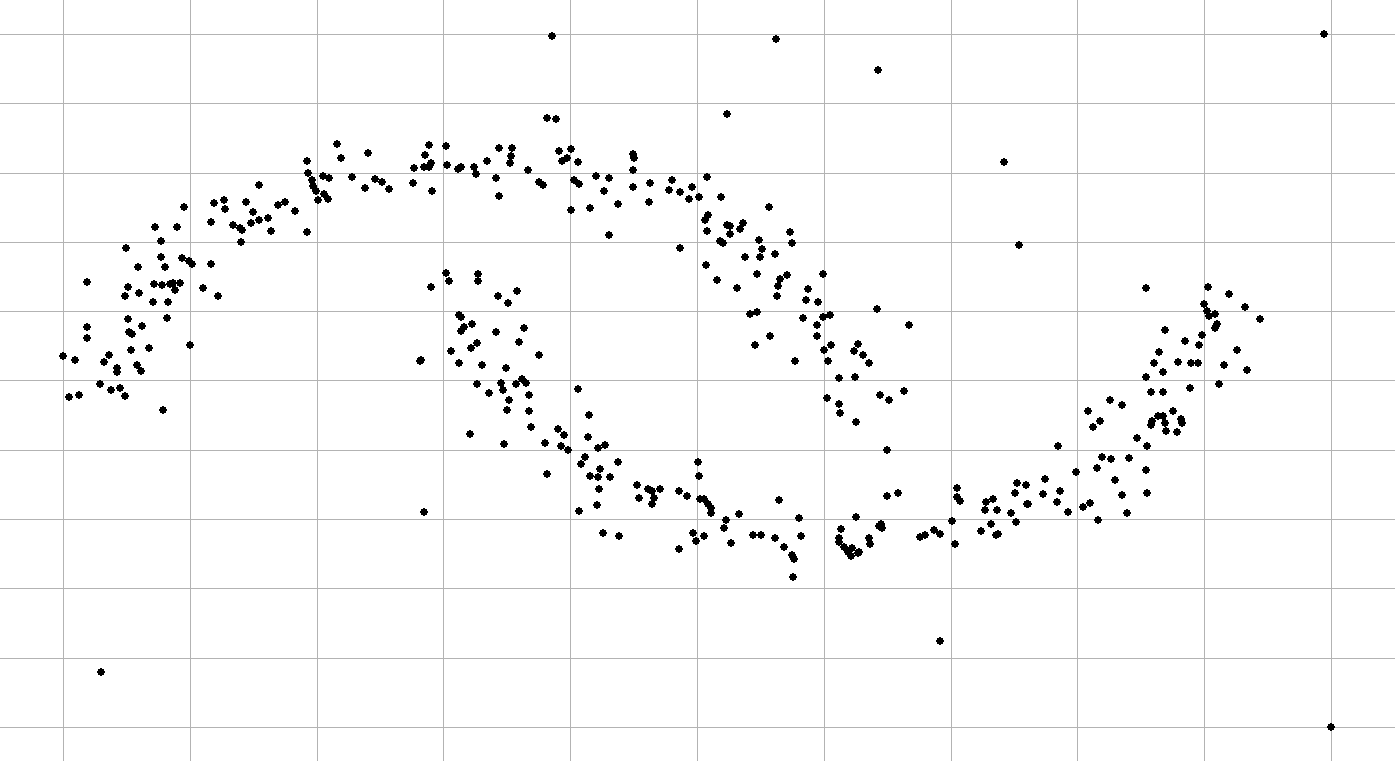
\includegraphics[width=0.8\linewidth]{Images/Grid construction.png}
		\caption{A dataset consisting of two non-spherical, moon-shaped clusters and random noise, partitioned into a 10×10 grid using the described steps.
        \\And the dataset is generated by R with a rnorm function added to two half circles to be clusters. The outlier is generated by uniform distribution.}
	\end{figure}
    
    \begin{figure}[H]
		\centering
		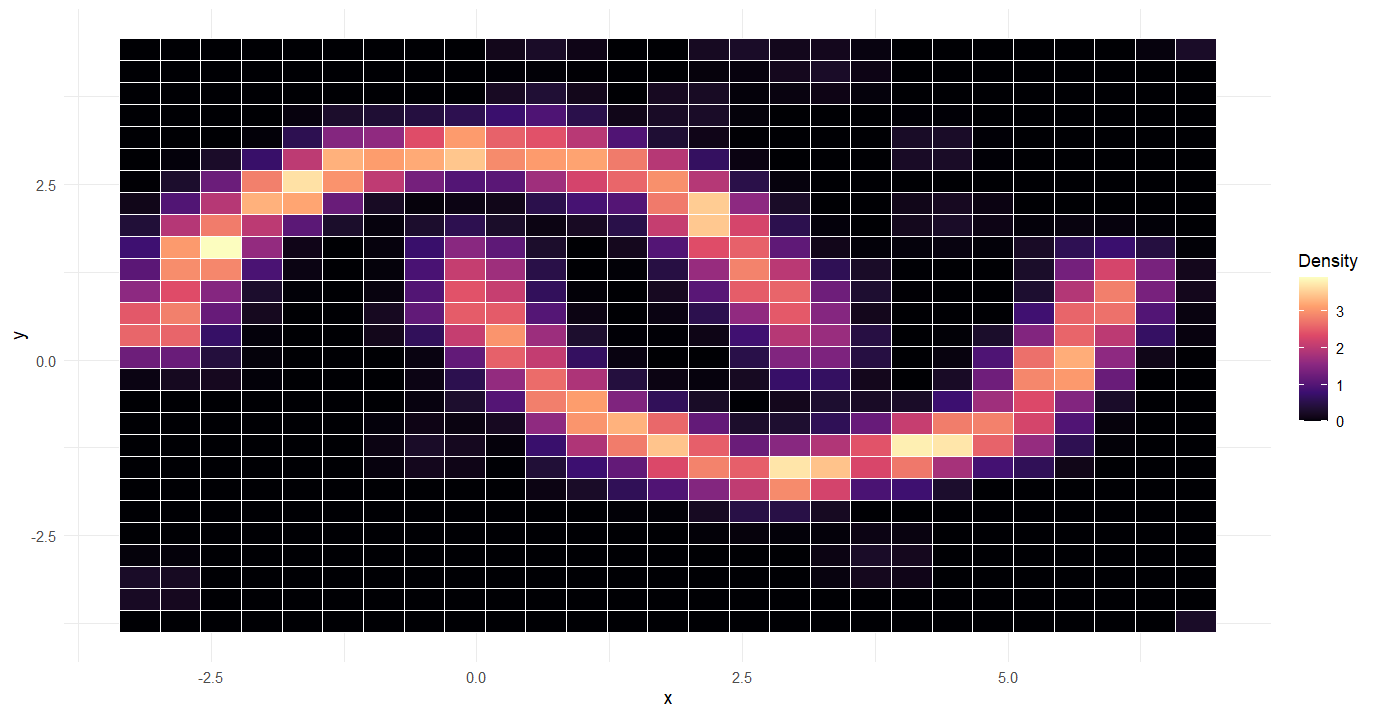
\includegraphics[width=0.8\linewidth]{Images/heat map.png}
		\caption{Heat map of the dataset provided, which shows where the data are concentrated under 27$\times$27}
	\end{figure}
	
	\columnbreak
	\subsection{2.2 Density Estimation}
    \vspace{-0.8cm} 
	\rule{\linewidth}{3pt} 
	\begin{enumerate}
		\item Calculate the relative proportional positions $t_x$ and $t_y$ (both within $[0,1]$) of a data point $(x,y)$ inside its primary hosting cell $[L_x, R_x] \times [L_y, R_y]$.
		
		\[
		t_x=\frac{x-L_x}{R_x-L_x}\quad,
		\qquad
		t_y=\frac{y-L_y}{R_y-L_y}
		\]
		
		\item Define vectors $W_x$ and $W_y$ along the $X$ and $Y$ axes, corresponding to the [left/lower neighbor, primary cell, right/upper neighbor].
		
    \[
    W_x = \left[ \frac{1 - t_x}{2},\; 0.5,\; \frac{t_x}{2} \right]
    \]
    \[
    W_y = \left[ \frac{1 - t_y}{2},\; 0.5,\; \frac{t_y}{2} \right]
    \]
		
		\item Compute the final density weight $W_{ab}$ allocated to each cell $Cell(a, b)$ within the neighboring 3x3 grid (nine-grid) via the outer product of $W_x$ and $W_y$ (Figure 2).
		
		\[
		W_{ab} = W_x[a] \times W_y[b], \quad a,b \in \{1,2,3\}
		\]
	\end{enumerate}


	\subsection{2.3 Cluster Formation and Outlier Detection}
    \vspace{-0.8cm} 
	\rule{\linewidth}{3pt}
Cells with a combined density $\geq thr$ are retained as ``surviving cells''. Two surviving cells are connected if their grid distance $\leq 1$ in both directions.(Figure 3) 

A data point is assigned to a connected grid if its contribution is $\geq 1/4$. Consequently, each connected grid component forms a distinct \textbf{cluster}, while any unassigned points are labeled as \textbf{outliers}.
	
	\columnbreak
    
	\subsection{2.4 Identify Best Grid Resolution and threshold}
	\vspace{-0.8cm} 
	\rule{\linewidth}{3pt}
	We introduce DBCV, which provides a more robust evaluation of clustering performance in datasets with irregular or non-spherical distributions.\cite{doi:10.1137/1.9781611973440.96}
	\par
	However, the DBCV does not 'punish' excessive outliers, which may lead to a big number of outliers that are close to the cluster but are not absorbed. So we introduce an Adjusted DBCV score: we subtract a number that is proportional to the outlier ratio to reduce the potential possibility of too many outliers.
	\par
	For bigger Adjusted DBCV values, the cluster fits better, so we return the corresponding clusters and outliers.(Figure 4)
	
	\[
	\mathrm{Adjusted\;DBCV} = \mathrm{Raw\;DBCV} - \beta \times r_{\mathrm{outlier}}
	\]
	\[
	r_{\mathrm{outlier}} = \frac{N_{\mathrm{outlier}}}{N_{\mathrm{points}}}
	\]
    
	\begin{figure}[H]
		\centering
		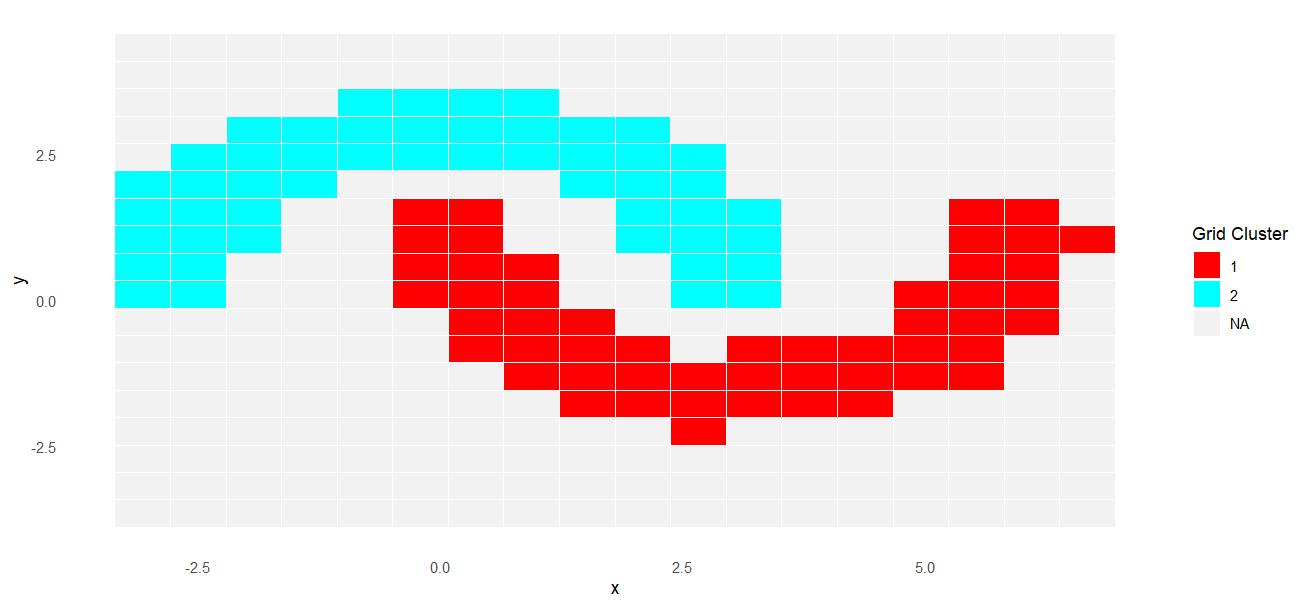
\includegraphics[width=0.7\linewidth]{Images/grid.png}
		\caption{Connected cells according to combined density.}
	\end{figure}	
    
	\begin{figure}[H]
		\centering
		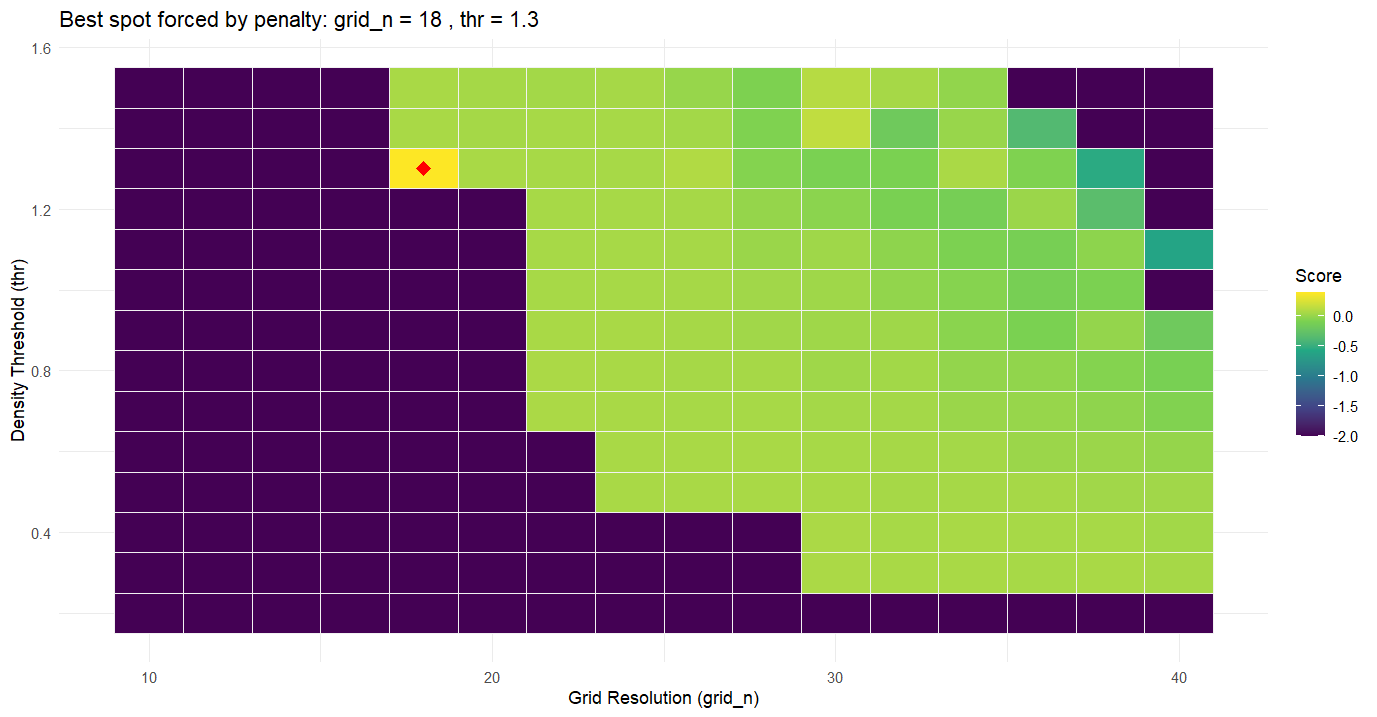
\includegraphics[width=0.7\linewidth]{Images/DBCV.png}
		\caption{Adjusted DBCV values respecting to different $thr$ and grid\_n values, diamond indicates the best grid\_n and $thr$.}
	\end{figure}
    
    \columnbreak
    
	\section{3. Strengths and Limitations}
	\vspace{-2.5cm} 
	\rule{\linewidth}{3pt}
	Our method fits well for non-spherical datasets, and it can automatically identify outliers. Whereas K-means and hierarchical clustering does not.(Table 1, Figure 5)
	\par
	However, the algorithm performs excellently in 2D space but struggles to scale to high-dimensional spaces. Because the grid is partitioned strictly along the coordinate axes, a $10 \times 10$ splitting yields only 100 cells in 2D space, but escalates to $10^3 = 1000$ cells in 3D space. If the data scales to $D$ dimensions, the number of cells explodes exponentially to $10^D$.

	\begin{table}[H] 
		\centering 
		\footnotesize 
		\caption{ARI of different methods.} 
		\begin{tabular}{lc} 
			\toprule
			Method & ARI \\
			\midrule
			Grid Density & 0.9709 \\
			K-means & 0.2542 \\
			Hierarchical clustering & 0.238 \\
			\bottomrule
		\end{tabular}
	\end{table}
	
	\begin{figure}[H]
		\centering
		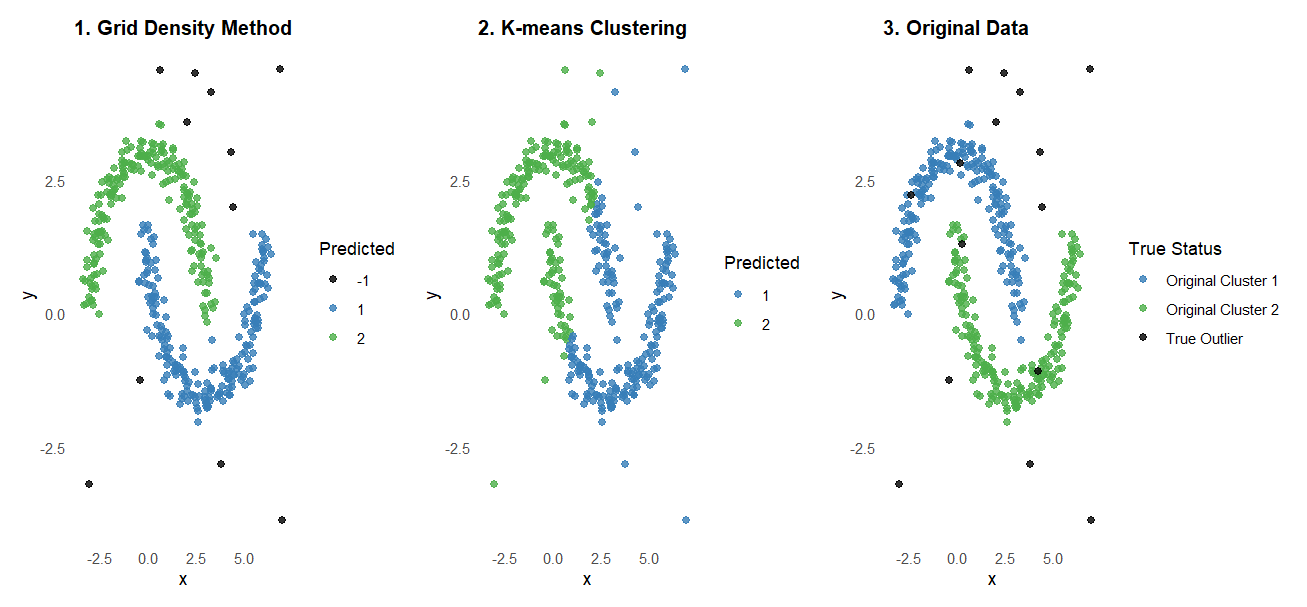
\includegraphics[width=\linewidth]{Images/comparison.png}
		\caption{A comparison of row dataset to Cell Density-Based Grid Clustering and K-means, black dots represents the outliers.}
	\end{figure}
	
	{\small
\bibliographystyle{plain}
\bibliography{siam_1.9781611973440.96}
}

\end{multicols}

\end{document}
